% !TeX spellcheck = en_US
\subsection{Non-Equilibrium Work\label{Sec:FEM:NEW}}
Non-Equilibrium Work (NEW) method for equilibrium free energy calculations was firstly proposed by Jarzynski.\cite{JarzynskiPRL1997}. 
In 1997, Jarzynski showed
\begin{equation}
\left< \exp\left[-\beta W(\tau)\right] \right> = \exp{(-\beta \Delta A)},
\label{Eq:FEM:NEW:Jar}
\end{equation}
which is now called the Jarzynski equality. Here, $W$ is the accumulated work along a path $\lambda(t)$ connecting the initial and final states, with $\lambda(0)=0$ and $\lambda(\tau)=1$, and $\Delta A = A(1) - A(0)$ the free energy difference between these two states. 
$\left \langle \cdots \right \rangle$ in Eq.~\ref{Eq:FEM:NEW:Jar} is an average over a series of trajectories with the initial conditions chosen according to the equilibrium Boltzmann probability in state $\lambda(0)$. The path average samples all the realizations of dynamic paths weighted by their respective path actions under the time evolution of the system with an explicitly time-dependent Hamiltonian. This equality was also obtained by Crooks for markovian and microscopically reversible dynamics.\cite{CrooksJSP1998} 

Now, we consider creating an equilibrium configuration for the state $\lambda=0$ and then slowly changing $\lambda$ from 0 to 1. As the coupling parameter is advanced, the system continues to sample phase space by molecular dynamics or Monte Carlo simulations, but under an explicitly time-dependent Hamiltonian. In the limit of a very slow transformation, with some caveats of Hamiltonian dynamics, the system will remain close to the equilibrium. The free energy difference can then be evaluated by changing $\lambda$ continuously
\begin{equation}
\Delta A =\lim_{\tau\to\infty} \int_{0}^{\tau} {\frac{\partial{H\left[\textbf{x}(t);\lambda\right]}}{\partial{\lambda}}\bigg\rvert}_{\lambda=\lambda(t)} \dot{\lambda}(t) dt,
\label{Eq:FEM:NEW:limitA}
\end{equation}  
where $\dot{\lambda}(t)$ is the time derivative of the coupling parameter $\lambda$. In Eq.~\ref{Eq:FEM:NEW:limitA}, the limit of $\tau\to\infty$ ensures that the transformation is performed infinitely slowly, and thus reversibly. The right-hand side of Eq.~\ref{Eq:FEM:NEW:limitA} is the ``reversible work'' done to the system during the transformation.

If the system is instead transformed between the initial and final states over a finite time interval $\tau$, the system will not be able to sample the phase space exhaustively at each value of $\lambda$, making this transformation irreversible. As the transformation proceeds, the system will be gradually driven out of equilibrium, causing hysteresis effects. From the second law of thermodynamic, it is expected that the work $W(\tau)$ performed during the nonequilibrium transformation is on average larger than or equal to the free energy difference between the two states
\begin{equation}
\left \langle W(\tau) \right \rangle \ge \Delta A,
\label{Eq:FEM:NEW:WA}
\end{equation} 
and the difference accounts for heat-dissipation effect. The work $W(\tau)$ performed on the system is the accumulated energy cost required to change the system
\begin{equation}
W(\tau) = \int_{0}^{\tau} \frac{\partial{H[\textbf{x}(t);\lambda]}}{\partial{\lambda}}\bigg\rvert_{\lambda=\lambda(t)} \dot{\lambda}(t) dt
\label{Eq:FEM:NEW:work}
\end{equation}    
The equality in Eq.~\ref{Eq:FEM:NEW:WA} will normally be achieved only if the transformation is infinitely slow, $\tau\to\infty$.  For paths of finite length, the amount of dissipated work, $\left \langle W(\tau) \right \rangle - \Delta A \ge 0$, depends on the chosen transformation path $\lambda(t)$.

Jarzynski equality, Eq.~\ref{Eq:FEM:NEW:Jar}, immediately leads to the second law in the form of Eq.~\ref{Eq:FEM:NEW:WA} because of the Jensen's inequality, $\left \langle e^{-x} \right \rangle \ge e^{-\left<x\right>} $.
Moreover, TI and TP can be thought as the limiting cases of the nonequilibrium process. When $\tau\to\infty$ or $\dot{\lambda}(t)\to0$, this is an infinitely slow transformation and the Eq.~\ref{Eq:FEM:NEW:limitA} is the formula of TI
\begin{equation}
\Delta A = \int_{\lambda=0}^{\lambda=1}\left \langle \frac{\partial{H(\textbf{x},\textbf{p}_{x},\lambda)}}{\partial{\lambda}} \right \rangle_{\lambda} d\lambda
\label{Eq:FEM:NEW:TINEW}
\end{equation}  
When $\tau\to0$ or $\dot{\lambda}(t)\to\infty$, this is an infinitely fast transformation where the configurations will not relax and the work is simply the change in the Hamiltonian when going from the initial to the final state,
\begin{equation}
\lim_{\tau\to0}W(\tau) = H(\textbf{x}(0);\lambda=1)-H(\textbf{x}(0);\lambda=0)
\label{Eq:FEM:NEW:limitW}
\end{equation}
Substituting the Eq.~\ref{Eq:FEM:NEW:limitW} into the Eq.~\ref{Eq:FEM:NEW:Jar}, the formula of TP can be recovered
\begin{equation}
\Delta A = -\frac{1}{\beta} \ln \left \langle \exp[-\beta \Delta H(\textbf{x},\textbf{p}_{x})] \right \rangle  _{0},
\label{Eq:FEM:NEW:deltaA4NEW}
\end{equation}

\begin{figure}[htbp]
	\centering
	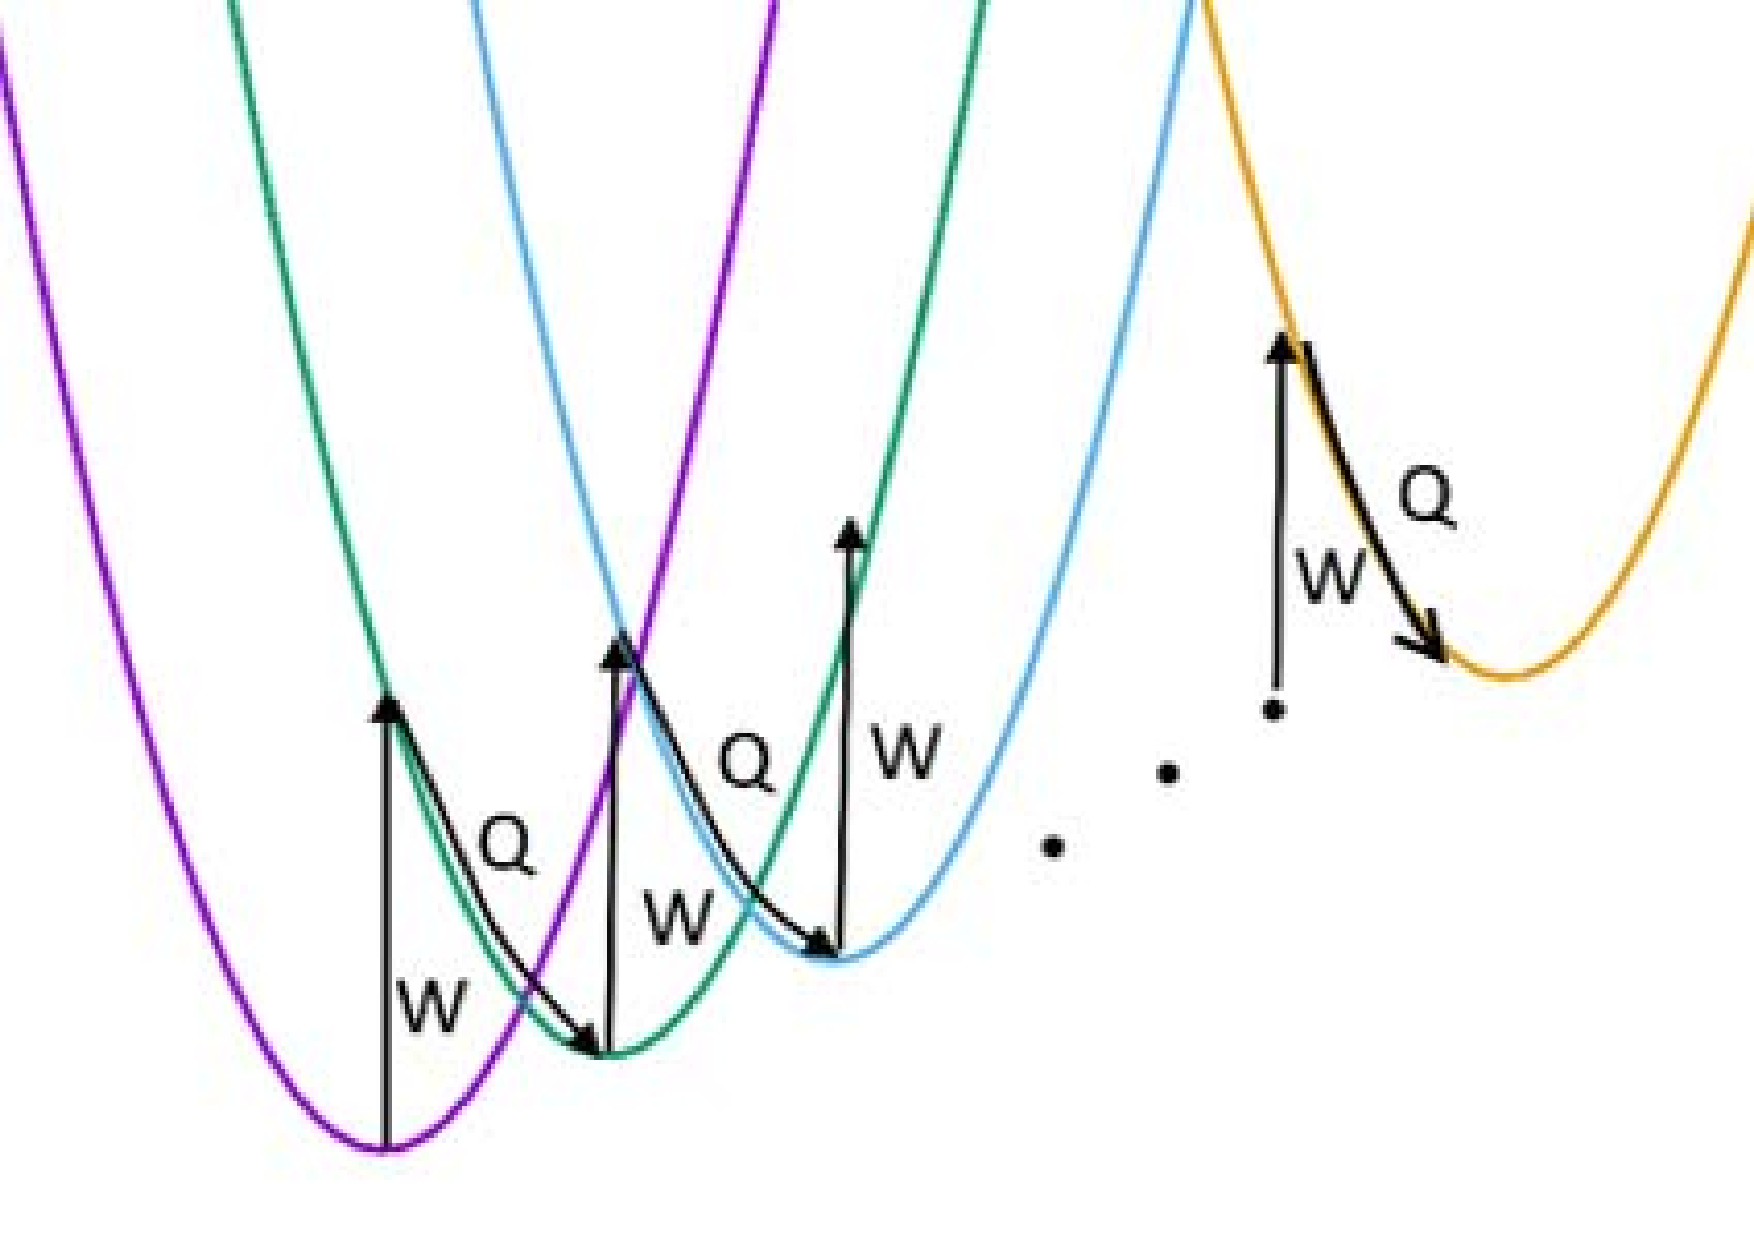
\includegraphics[width=0.4\textwidth]{figures/NEW.pdf}\\
	\caption{The accumulation of work and heat along a nonequilibrium trajectory. The work is defined as the energy change when the coupling parameter switches from $\lambda_i$ to $\lambda_{i+1}$ with the coordinates fixed, while the dissipated heat is defined as the energy relaxation when the coordinate change with the coupling parameter fixed.}\label{Fig:FEM:NEW}
\end{figure}

In Ref.~\cite{CrooksJSP1998}, Crooks showed that the distributions of work values from the forward and the backward paths satisfy a relation that is central to the histogram methods in free energy calculations
\begin{equation}
\frac{p_{f}[w=W(\tau)]}{p_{b}[w=-\underline{W}(\tau)]}=\exp[\beta(w-\Delta A)],
\label{Eq:FEM:NEW:crooks}
\end{equation}
where $p_{f}[w=W(\tau)]$ and $p_{b}[w=-\underline{W}(\tau)]$ are the probability densities of the work values in the forward and the reverse transformations (with a sign change for the work in the reverse path). Both are normalized, i.e., $\int p_{f}(w) dw=\int p_{b}(w) dw=1$. It is noted that Jarzynski equality Eq.~\ref{Eq:FEM:NEW:Jar} follows from Eq.~\ref{Eq:FEM:NEW:crooks} simply by integration over $w$ because the probability densities are normalized to 1:
\begin{equation}
\int p_{f}(W)e^{-\beta W}dW=\int p_{b}(W)e^{-\beta \Delta A}dW,
\label{Eq:FEM:NEW:crookstojar}
\end{equation}
Because of the normalization condition, the right-hand side is equal to $\exp(-\beta \Delta A)$, and Jarzynski equality follows.

Following the Crooks Fluctuation Theorem (CFT),\cite{CrooksJSP1998} Bennett acceptance ratio can be applicable to nonequilibrium calculations. This approach was combined with a maximum likelihood estimate, and accurate free energy differences were obtained.\cite{ShirtsPRL2003}
In this approach, $\Delta A$ is calculated via
\begin{align}
\sum_{i=1}^{n_{F}}\frac{1}{1+\exp \left[\beta(M+W_{i}-\Delta A)\right]} = \sum_{j=1}^{n_{R}}\frac{1}{1+\exp \left[-\beta(M+W_{j}-\Delta A)\right]},
\label{Eq:FEM:NEW:NEBAR}
\end{align}
where $n_{F}$ and $n_{R}$ are the numbers of the forward and reverse transformations respectively, $W_{i}$ and $W_{j}$ are the work of forward and reverse measurements respectively, and $M=\beta^{-1}$ln($n_{F}$/$n_{R}$).
The corresponding statistical variance of $ \Delta A $, $ \sigma^2 $, is calculated using Eq.~10 in Ref.~\cite{ShirtsPRL2003}.